% Make a complete abstract

The PyCBC Live early warning search identifies \gwadj signals prior to merger, giving warning to the international astronomy community of an incoming \gwadj event. The early warning search is an adaptation to the PyCBC Live full bandwidth search---discussed heavily in chapter~\ref{chapter:5-pycbc-live}---and we have identified problems relating to search for pre-merger signals which require changes to be made to the early warning infrastructure to improve the sensitivity of the pipeline.

In section~\ref{6:sec:multi-messenger-astronomy} we discuss the joint detection of astrophysical events with both \gw and electromagnetic observatories, in section~\ref{6:sec:gw170817} we highlight the only multi-messenger event seen thus far and the timeline of observations. The PyCBC Live early warning search is described in section~\ref{6:sec:early-warning-search} with the template bank construction in section~\ref{6:sec:early-warning-template-bank} and how sky localisation for events is obtained in section~\ref{6:sec:event-localisation}. Section~\ref{6:sec:gw170817-in-ew} uses GW1701817 as an example to demonstrate the capabilities of the early warning search and in section~\ref{6:sec:injection-tests} we describe a full injection set test performed using the early warning search to identify any problems and the results of this search. Finally in section~\ref{6:sec:identified-problems} we discuss the problems found when testing the early warning search, the cause of the problems and the potential solutions to these problems.

\section{\label{6:sec:multi-messenger-astronomy}Multi-messenger astronomy}

The PyCBC \gwadj search pipeline searches for \gwadj signals from the merger of two compact objects~\cite{PyCBC:2016}. Black holes do not emit electromagnetic radiation and therefore the merger of two black holes can currently only be directly observed with \gwadj detectors~\cite{Ghez:2000}. Neutron stars, on the other hand, are electromagnetically bright themselves and the merger of two neutron stars will produce a kilonova~\cite{Kilonovae:2017}. Kilonovae emit a broad range of electromagnetic radiation across the spectrum~\cite{kilonova_lightcurve:2017} which can be observed with many of the ground and space-based electromagnetic observatories we have on Earth. The combination of \gw and electromagnetic emissions allows us to understand more about these events than either observation could provide alone~\cite{multi_mess_astro:2019}. Astrophysical events which have been observed with more than one type of signal are called multi-messenger events, this can be from any of the three: electromagnetic signals, \gws or neutrinos. We will use the term `multi-messenger event' to describe an event which has been seen with a \gwadj signal and an electromagnetic counterpart.

One such quantity that can be measured from observing kilonovae with both \gws and electromagnetic radiation is the Hubble constant~\cite{Schutz:1986}, the measured rate of expansion of the Universe~\cite{hubble:1929}. The Hubble constant is currently determined across two distance scales using purely electromagnetic observations: firstly, the large scale cosmological measurements using the cosmic microwave background~\cite{WMAP_H0:2003} and baryon acoustic oscillations~\cite{BAO_H0:2009} and secondly, the local Universe scale using the astrophysical standard candle Cepheid variable stars~\cite{Cepheids_H0:2001} and type Ia supernovae~\cite{TypeIa_H0:1998}. The Hubble constant values obtained at the different scales do not agree~\cite{H0_tension:2020} so by combining the observation of binary neutron star signals using both \gw and electromagnetic observatories we can provide an independent measurement of the Hubble constant to break this tension.

At nearby distances ($d \lesssim 50 \, \text{Mpc}$) the Hubble constant can be approximated using Hubble's law~\cite{hubble:1929},
%
\begin{equation}
    v = H_{0} d,
    \label{6:eq:basic_hubbles_law}
\end{equation}
%
where $v$ is the recessional velocity of a source, $H_{0}$ is the Hubble constant and $d$ is the proper distance to the source. For nearby objects ($z \lesssim 0.1$): $v$ can be approximated as $v \approx cz$, where $z$ is the redshift of the object and $c$ is the speed of light; luminosity distance is approximately equal to the proper distance $d \approx D_{L}$. On small distance scales the expansion of the universe doesn't greatly affect these measurements. We obtain an equation for the Hubble constant at short distances
%
\begin{equation}
    H_{0} = c \frac{z}{D_{L}}.
    \label{6:eq:hubbles-law}
\end{equation}
%

The expansion rate of the Universe historically is not constant. For objects at larger distances we have to account for redshift in the luminosity distance. We begin by defining the luminosity distance in terms of the comoving distance
%
\begin{equation}
    D_{L}(z) = (1 + z)D_{c}(z),
\end{equation}
%
which accounts for the expanding universe in the term $(1 + z)$. The comoving distance is given by
%
\begin{equation}
    D_{c}(z) = c \int^{z}_{0} \frac{dz^{\prime}}{H(z^{\prime})},
\end{equation}
%
where the Hubble constant, $H(z^{\prime})$, is now the Hubble parameter at redshift $z^{\prime}$ and depends on the model of cosmology.
We can use the comoving distance to get an expression for the luminosity distance,
%
\begin{equation}
    D_{L}(z) = (1 + z) c \int^{z}_{0} \frac{dz^{\prime}}{H(z^{\prime})}.
\end{equation}
%
$H_{0}$ will depend on the cosmological parameters representing the density of matter, radiation and dark energy. To measure the Hubble constant we need to measure the redshift and luminosity distance of multiple sources.

The luminosity distance of a \gwadj event is inversely proportional to the amplitude of the \gwadj strain~\cite{Schutz:1986},%
\begin{equation}
    h(t) \propto \frac{1}{D_{L}} , 
\end{equation}
%
which is obtained via \gwadj searches and parameter estimation. The \gwadj strain amplitude does have a degeneracy with the inclination angle, $\iota$, of the binary neutron star system which is described as the angle between the line of sight to the observer and the orbital angular momentum of the source~\cite{inclin_degen_2:2019}.

The \gwadj strain dependence on inclination angle manifests differently in the two \gwadj polarisations and can be simply described as~\cite{inclin_degen:2018},
%
\begin{align}
    h_{+} &\propto \left(1+\cos^{2}\iota\right), \\
    h_{\times} &\propto \cos\iota .
    \label{6:eqn:inclin_polarisations}
\end{align}
%
It can be seen from equation~\ref{6:eqn:inclin_polarisations} that an edge-on system ($\iota = 90^{\circ}$) will produce a signal entirely in the $h_{+}$ polarisation but an face-on system will produce a mixed signal with contributions from both $h_{+}$ and $h_{\times}$. The inclination angle degeneracy could be broken if we were able to measure $h_{+}$ and $h_{\times}$ independently but the individual \gwadj detectors are sensitive only to a linear combination of the polarisations~\cite{aLIGO:2015}. Multiple \gwadj detectors with different orientations will be sensitive to different linear combinations of $h_{+}$ and $h_{\times}$ and are therefore required to break this degeneracy and fully reconstruct the source orientation~\cite{inclin_degen_2:2019}.

To measure the redshift of the event using the \gwadj signal we can look to the chirp rate of the system. 


The chirp rate is defined as the rate of charge of the \gwadj frequency,
% %
% \begin{equation}
%     \frac{1}{2\pi} \Dot{\Phi}(t_{f}) = f,
% \end{equation}
% %
% where $\Dot{\Phi}(t_{f})$ is the rate of change of the orbital phase at time $t_{f}$ at which the instantaneous frequency of emitted radiation is equal to the frequency $f$. We know the orbital and waveform phase are related by
% %
% \begin{align}
%     \phi_{gw} = 2\phi(t),
% \end{align}
% %
% as well as to the orbital angular frequency
% %
% \begin{equation}
%     \Dot{\phi} = \frac{1}{2}\omega,
% \end{equation}
% %
% where
% %
% \begin{equation}
%     \Dot{\omega}_{gw} = \frac{12}{}
% \end{equation}


The chirp rate to Newtonian order is given by
%
\begin{equation}
    \frac{df}{dt} = \frac{96}{5} \pi^{8/3} \left(\frac{G\mathcal{M}}{c^{3}}\right)^{5/3} f^{11/3},
    \label{6:eq:chirp_rate}
\end{equation}
%
the rate of change of the \gwadj frequency is easy to measure and will give us the chirp mass of the system,
%
\begin{equation}
    \mathcal{M} = \frac{(m_1 m_2)^{\frac{3}{5}}}{(m_1 + m_2)^{\frac{1}{5}}}.
    \label{6:eq:mchirp}
\end{equation}
%
which depends on the two masses of the system, $m_{1}$ and $m_{2}$. In \gwadj searches we use 3.5PN order corrections to the wavefor\footnote{See section~\ref{1:sec:post_newtonian_treatment} for further information.}.

The observed $\mathcal{M}$ is redshift dependent,
%
\begin{equation}
    \mathcal{M}_{obs} = \mathcal{M}_{source}(1 + z), 
    \label{6:eq:mchirp_obs}
\end{equation}
and $\mathcal{M}_{obs}$ is scaled by the redshift where events with larger redshifts will appear with larger observed chirp masses than their source chirp mass, $\mathcal{M}_{source}$. We would require a measurement of the Hubble constant to determine the redshift using the luminosity distance and we reach a circular argument.

We can look at other ways to measure the redshift of the event without using the \gwadj signal. The primary candidate is an electromagnetic emission from the event, for example, a kilonova from a binary neutron star system. Using the electromagnetic emission we can locate the host galaxy of the source and find the approximate redshift of the binary neutron star system. We will then have a luminosity distance, measured by the \gwadj signal, and a redshift, measured by the electromagnetic observation, and using equation~\ref{6:eq:hubbles-law} we can calculate the Hubble constant . This combination of event information from two separate sources of information for the same event means we can use electromagnetically bright \gwadj sources as another standard siren for measuring the Hubble constant, highlighting the importance of observing multi-messenger events.

\section{\label{6:sec:gw170817}GW170817: The only multi-messenger event}

We have described multi-messenger events as those that have been seen with a \gw and an electromagnetic signal, in reality the event will broadcast information across the electromagnetic spectrum at varying timescales so we might see a single \gwadj signal but multiple electromagnetic signals. We have observatories around the globe and in space which span this entire spectrum and can observe counterparts to our \gwadj signal in all of the different frequency ranges: from high frequency gamma rays to long wavelength radio waves. 

GW170817~\cite{GW170817:2017} is the first and only multi-messenger event we have observed, the Q-scans depicting the \gwadj signal found by the three detectors online at the time of the event can be seen in figure~\ref{6:fig:gw170817_qscan} and the GCN circular~\cite{gcn_circulars:2024} (rapid astronomical bulletins submitted by and distributed to the global physics community) can be found at: \href{https://gcn.gsfc.nasa.gov/other/G298048.gcn3}{https://gcn.gsfc.nasa.gov/other/G298048.gcn3}. On the 17th August 2017 at precisely 12:41:04 UTC the \gws from the merger of a binary neutron star system were seen by LVK detectors. Only $1.7$ seconds later a gamma-ray burst (GRB 170817A~\cite{gw170817_joint:2017}) was seen by Fermi~\cite{Fermi:2022, Fermi_GW170817:2017} and INTEGRAL~\cite{INTEGRAL:2003, INTEGRAL_GW170817:2017}. The kilonova emissions were seen next, visual light by the Hubble Space Telescope (HST)~\cite{HST:2000, HST_GW170817:2021} at 11 hours, infrared by HST, VISTA~\cite{VISTA:2015, VISTA_GW170817:2017} and Spitzer~\cite{Spitzer:2004, Spitzer_GW170817:2018} at 12 hours and UV by Swift's UVOT~\cite{Swift:2004, Swift_GW170817:2017} at 15.3 hours post-merger. The final electromagnetic frequencies to be seen were X-rays by Chandra~\cite{Chandra_GW170817:2017} at 9 days post-merger and radio waves by VLA~\cite{VLA:2019, VLA_GW170817:2017} at 16 days post-merger.
%
\begin{figure}
    \centering
    \includegraphics[width=0.8\linewidth]{images/6_earlywarning/gw170817/GW170817_qscan.pdf}
    \caption{The three detector (LIGO-Hanford (top), LIGO-Livingston (middle) and Virgo (bottom)) time-frequency images (Q-scan~\cite{qscan:2004} showing data containing the first binary neutron star \gwadj event, GW170817~\cite{GW170817:2017}, with times shown relative to 17th August 2017 12:41:04 UTC. The detector amplitudes are individually normalised for that detector's amplitude spectral density. The glitch observed in the LIGO-Livingston detector has been subtracted, the technique and results when doing so are presented in section IV of~\cite{GW170817:2017} and this figure is taken directly from figure 1 in~\cite{GW170817:2017}.}
    \label{6:fig:gw170817_qscan}
\end{figure}
%

Analysing GW170817's \gwadj signal and electromagnetic emissions reveal a binary neutron star system located in the Hydra constellation belonging to the galaxy NGC 4993~\cite{NGC4993:1998}. Using these signals the Hubble constant can be inferred as $H_0 = 70.0^{+12.0}_{-8.0} \, \text{km} \, \text{s}^{-1} \,\text{Mpc}^{-1}$~\cite{GW170817_H0:2017} which is consistent with both the measured cosmological value for $H_0$ ($67.74 \pm0.46 \, \text{km} \, \text{s}^{-1} \,\text{Mpc}^{-1}$~\cite{Planck_H0:2015}) and the astrophysical value for $H_0$ ($73.24 \pm1.74 \, \text{km} \, \text{s}^{-1} \,\text{Mpc}^{-1}$~\cite{Riess_H0:2016}) but, it is not accurate enough to break the tension between both values. To constrain the value of the Hubble constant further we need to observe many more electromagnetically bright events~\cite{Palmese:2021}. Using GW170817 we were able to determine other physical properties such as the speed of gravity~\cite{Harry_speed_of_gravity:2022, Baker_speed_of_gravity:2022}.

Using the electromagnetically bright multi-messenger events to constrain the measurement of the Hubble constant is straight forward. We are also able to use `dark siren' events, which have no electromagnetic counterpart and so rely entirely on the \gwadj emission to measure the redshift.


to measure the value of the Hubble constant 




we must use galaxy catalogues to locate the host galaxy of the \gwadj signal to obtain a redshift measurement. This is not discussed further in this chapter, for more information on dark sirens please look to~\cite{DES:2019, Dalang_dark_sirens:2023}

\section{\label{6:sec:early-warning-search}Detecting \gwadj events pre-merger}

\Gwadj signals from low-mass sources merge at a frequencies above the sensitive frequency band of the LIGO \gwadj detectors, therefore they are found at the Nyquist frequency of the LIGO detectors, ${\sim}1024 \, \text{Hz}$. The lower sensitive frequency of the LIGO detectors is ${\sim}20 \, \text{Hz}$ meaning the \gwadj signal can exist in the sensitive band for potentially hundreds of seconds before it is identified by the \gwadj search pipelines.

This presents an opportunity to detect the \gwadj signal pre-merger, in the inspiral regime of the system. The electromagnetic counterpart to the \gwadj signal all occurred post-merger, therefore by disseminating information about an on-going \gwadj event prior to the merger we are able to give enough warning to electromagnetic observatories to slew their telescopes to the approximation region on the sky in which we will indicate a \gwadj event will occur. Providing this warning pre-merger is commonly referred to as `early warning'. This section details the methodologies used in the PyCBC Live early warning search to achieve the detection of electromagnetically bright \gwadj signals pre-merger.

Even with an accurate sky map and dedicated electromagnetic telescopes (for example, GOTO is used for \gwadj event followup~\cite{GOTO:2020}), the gamma-ray burst counterparts can arrive less than two seconds after merger, not giving us enough time to identify the signal, produce a sky map and slew any telescopes to the correct sky location.

\subsection{\label{6:sec:pycbc-ew-search}The PyCBC Live early warning search}

PyCBC Live currently has two active configurations running on \gwadj data in real time: the full-bandwidth search aims to identify all \gwadj signals in the data in low-latency; the early warning search aims to identify potentially and circulate electromagnetically bright signals prior to their merger.

The PyCBC Live full bandwidth and early warning searches are very similar due to their use of the same infrastructure and code with a few key changes to enable as little latency between observable signal and circulation. The full bandwidth search uses an analysis stride of eight seconds, meaning new data is loaded and analysed every eight seconds, while the early warning search has an analysis stride of only one second.

We use two terms when referring to search detection times: latency refers to time taken by the search to identify a \gwadj template and produce a \gwadj event; and warning refers to the time prior to the \gwadj signal's merger that the event was identified. Figure~\ref{6:fig:latency_plot} shows the full bandwidth search which searches for complete templates and has a minimum and maximum latency of $12$ to $20$ seconds respectively with no possibility to observe the event pre-merger. The early warning search searches for templates that end pre-merger with minimum latency of $2.5$ seconds and maximum latency of $3.5$ seconds.
%
\begin{figure}
    \centering
    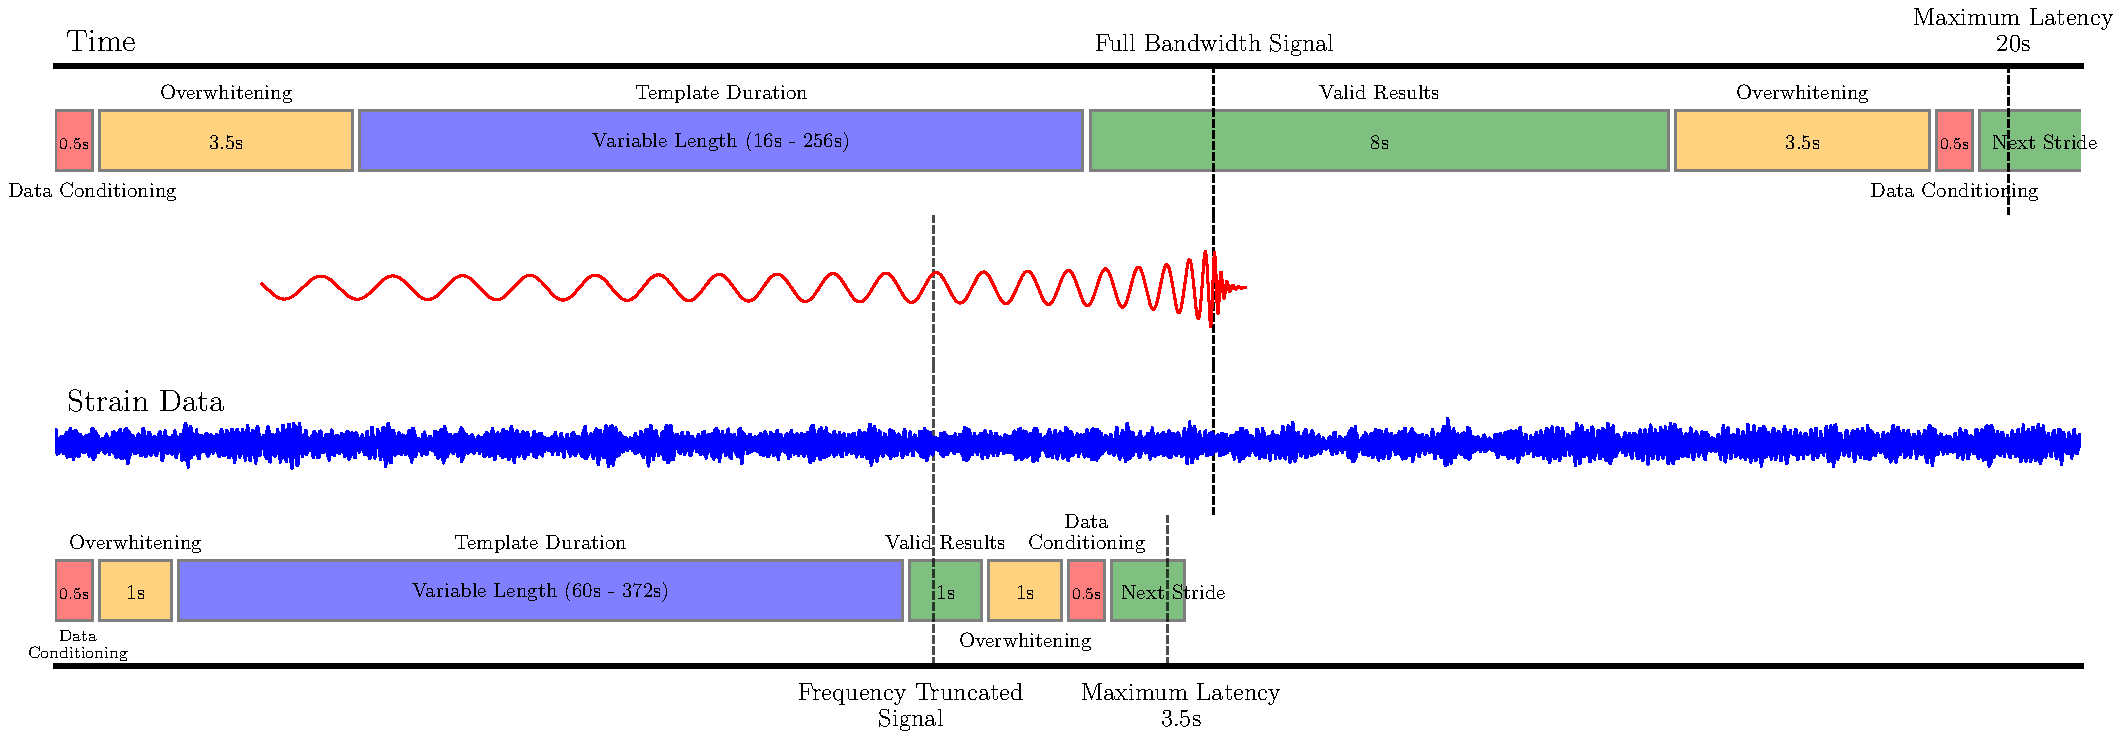
\includegraphics[width=\textwidth]{images/6_earlywarning/gw170817/latency_plot.pdf}
    \caption{An illustration of the detection latency between template end and event upload to GraceDB~\cite{ligo_gracedb:2024}. The top half of the plot pertains to the PyCBC Live Full Bandwidth search and indicates that the search has a maximum latency of $20$ seconds, the bottom half describes the PyCBC Live Early Warning search which has a maximum latency of $3.5$ seconds. From the end of the \gwadj template the search must wait for the current analysis stride to end, another period of data must then be waited on (overwhitening and data conditioning) and then the search analyses the previous analysis stride during the next analysis stride.}
    \label{6:fig:latency_plot}
\end{figure}
%
The early warning search is able to detect signal prior to the merger of the \gw and can give warning time whereas the full bandwidth search cannot.

The inspiral regime of the \gwadj signal is such that the frequency of the signal is monotonically increasing over time, to identify signals pre-merger the early warning search truncates the full \gwadj template at discrete frequency cutoffs and searches for these frequency truncated \gwadj templates. When a significant amount of SNR has been accumulated in the inspiral region the search will find the associated signal and predict the time of merger.

\subsection{\label{6:sec:early-warning-template-bank}Frequency truncated template bank}

The template bank used by the PyCBC Live early warning search is composed of frequency truncated templates. The bank contains six different frequency ctuoffs at: $29$, $32$, $38$, $44$, $49$ and $56 \, \text{Hz}$, these frequencies correspond to approximately $60$, $46$, $29$, $20$, $15$ and $10$ seconds before merger for a $1.4 \, \text{M$_\odot$}$\text{--}$1.4\, \text{M$_\odot$}$ binary neutron star signal and are shared between all the early warning pipelines: PyCBC Live~\cite{PyCBC_earlywarning:2020}, GstLAL~\cite{GstLAL:2020}, MBTA~\cite{MBTA:2021} and, SPIIR~\cite{SPIIR:2020}.

The PyCBC Live early warning template bank is constructed by generating six separate template banks (one for each frequency cutoff) using the standard geometric placement algorithm~\cite{Brown:2012} with a minimal match between templates of $0.97$; all six individual banks are then combined into one. The template parameters of the bank are chosen to represent potentially electromagnetically bright signals, these are produced by the merger of low mass binary neutron star or neutron star black hole systems. The masses of the two systems are limited between $1\text{--}3 \, \text{M$_\odot$}$, with no spins. The PSD used to generate the template bank is \verb|aLIGO140MpcT1800545| which is a representative PSD of the Advanced LIGO design curve that includes estimates for the main fundamental noises of the interferometer, in particular: seismic noise, thermal noise and quantum noise~\cite{aLIGO_design_curve:2018} with a binary neutron star range of $140 \, \text{Mpc}$~\cite{ligo_prospects:2016}.

The early warning template bank is $9180$ templates, making for a very light weight search when compared to the ${\sim}700,000$ templates being used in the full bandwidth PyCBC Live search. Not only are there fewer templates in the bank, the templates themselves are shorter in duration when compared to their full bandwidth counterparts in the full bandwidth template bank (but still quite long).
%
\begin{figure}
    \centering
    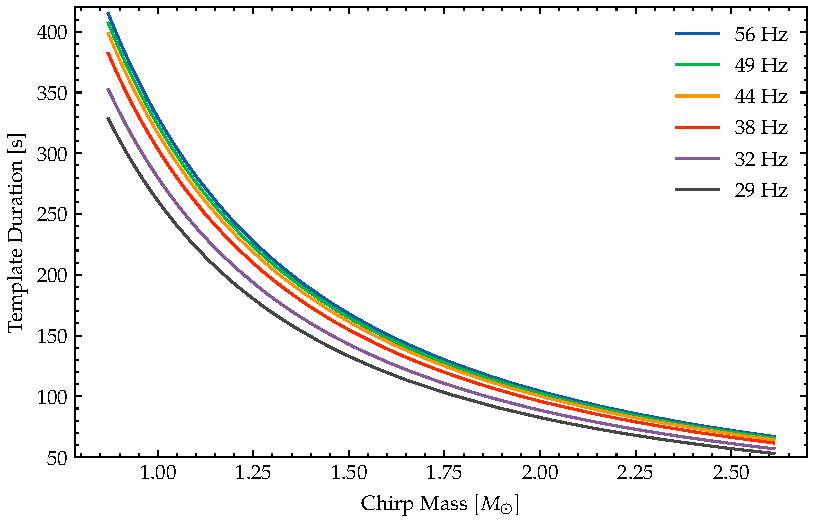
\includegraphics[width=\textwidth]{images/6_earlywarning/search/template_bank_duration_mchirp.pdf}
    \caption{Template duration versus chirp mass, $\mathcal{M}$, for different frequency cutoffs in the early warning template bank. Each curve corresponding to a different frequency cutoff, $f_{final}$, ($29\text{--}56  \, \text{Hz}$). The chirp mass is calculated from the component masses of the binary system, and the template duration is calculated between the lower frequency, $17 \, \text{Hz}$ and the frequency cutoff, $f_{final} \, \text{Hz}$.}
    \label{6:fig:tb_duration_mchirp}
\end{figure}
%
The duration of templates at each final frequency cutoff can be seen in figure~\ref{6:fig:tb_duration_mchirp} as a function of the chirp mass, $\mathcal{M}$, of the template. It can be seen that higher $\mathcal{M}$ templates have shorter duration and templates with a lower frequency cutoff also have shorter duration when compared to templates with the same $\mathcal{M}$ but a higher frequency cutoff.

\subsection{\label{6:sec:event-localisation}Determining event sky locations}

% (BRILLIANT PAGE FOR THIS https://emfollow.docs.ligo.org/userguide/early\_warning.html)

We call a \gwadj candidate obtained by the early warning search an `event'. These events have information about the \gwadj parameters and make a prediction of the time of coalescence of the \gwadj signal. Identifying the sky location of the event is critical for multi-messenger astronomy. With a sky location the \gwadj observatories are able to tell electromagnetic observatories where to slew their telescopes to see the event prior to merger, to have the best chance of seeing electromagnetic counterparts as possible.

The two parameters which describe the sky location are the right ascension and declination and the easiest way to measure these parameters are with time-of-arrival triangulation, measuring the time differences between time of arrivals at different detectors. The greater number of \gwadj detectors in the network lead to more accurate sky location triangulation. Figure~\ref{6:fig:gw170817_skymap} shows the sky map created for GW170817~\cite{gw170817_skymap:2017} with the source location identified by the LIGO-Hanford and LIGO-Livingston detectors shown in the green dashed contour (representing the 90\% confidence interval). Two detectors are limited to a ring on the sky but the detector quadrupolar sensitivity pattern of the antenna response will favour particular sky locations where the detector is more sensitive to \gws coming from certain angles. We can also use amplitude differences between the signal strength measured by each detector to determine the \gwadj polarisation which localizes sky location even further, giving not a ring but a broken ring on the sky map.
%
\begin{figure}
    \centering
    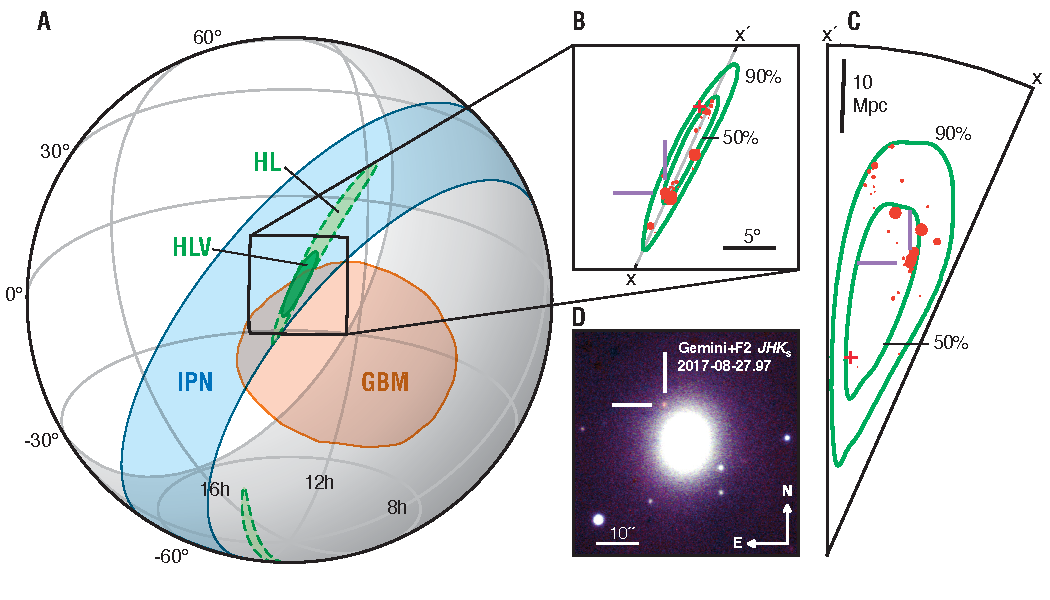
\includegraphics[width=1.0\linewidth]{images/6_earlywarning/gw170817/GW170817_skymap.pdf}
    \caption{The localisation of GW170817 and associated electromagnetic counterpart. The rapid LIGO localisation is indicated by the green dashed contour, and the LIGO \& Virgo localisation by solid green. Fermi~\cite{Fermi:2022} is shown in orange, and the Interplanetary Network triangulation from Fermi and INTEGRAL~\cite{INTEGRAL:2003} in blue. This figure is taken directly from~\cite{gw170817_skymap:2017}}
    \label{6:fig:gw170817_skymap}
\end{figure}
%

A greater number of detectors observing the event will produce more accurate sky locations; adding a third detector to the network (like Virgo~\cite{aVirgo:2015}) is required for a point sky location. BAYESTAR~\cite{BAYESTAR:2016} is a tool for providing accurate sky maps from \gwadj events in as little as a few seconds. As a \gwadj signal is observed by templates with higher and higher frequency cutoffs the sky map will become more accurate due to the increase in accumulated SNR. To demonstrate the improving sky map localisation as the signal progresses through our template bank we can produce the sky maps found by the early warning search when looking for a $1.4 \, \text{M$_\odot$}\text{--}1.4 \, \text{M$_\odot$}$ binary neutron star injection at a random point on the sky. The \gwadj injection is placed at a distance such that the full bandwidth SNR of the signal is $30$. Figure~\ref{6:fig:ew_30SNR_multiple} shows the sky map displaying the 90\% confidence interval contours for every frequency cutoff in the template bank as well as the full bandwidth sky map, the sky location of the injection can be seen as a star on the sky map. In the legend of the figure you can see the decreasing sky localisation area as frequency cutoff increases.
%
\begin{figure}
    \centering
    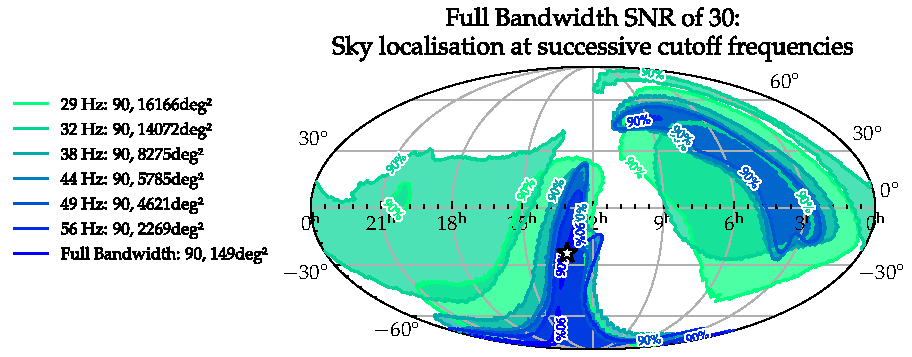
\includegraphics[width=\textwidth]{images/6_earlywarning/localisation/30SNR_multiple.pdf}
    \caption{The \gwadj sky localisation probability map (sky map) corresponding to a $1.4 \, \text{M$_\odot$}\text{--}1.4 \, \text{M$_\odot$}$ binary neutron star signal with a full-bandwidth (upper frequency cutoff $= 1024 \, \text{Hz}$) signal-to-noise ratio of $30$. The successive $90\%$ confidence interval sky map contours for frequency cutoffs from $29\text{--}56 \, \text{Hz}$ are shown where it can be seen that a higher frequency cutoff leads to a more accurate sky map.}
    \label{6:fig:ew_30SNR_multiple}
\end{figure}
%
\begin{table}[ht]
    \centering
    \setlength{\tabcolsep}{4pt}
    \rowcolors{4}{white}{lightgray}
    \begin{tabular}{cccc}
        \toprule
        \textbf{Full SNR} & \textbf{10} & \textbf{20} & \textbf{30 (Fig.~\ref{6:fig:ew_30SNR_multiple})} \\
        \midrule
        \textbf{Frequency [Hz]} & \multicolumn{3}{c}{\textbf{Localisation area [deg$^{2}$] (90\% credible area) }} \\
        \cmidrule(lr){2-4}
        29 & Not Found & 26,583 & 16,166 \\
        32 & Not Found & 22,464 & 14,072 \\
        38 & Not Found & 12,303 & 8,275 \\
        44 & 18,584 & 8,408 & 5,785 \\
        49 & 14,068 & 6,758 & 4,621 \\
        56 & 9,636 & 4,679 & 2,269 \\
        1024 & 1,908 & 300 & 149 \\
        \bottomrule
    \end{tabular}
    \caption{The sky localisation areas found by BAYESTAR~\cite{BAYESTAR:2016} for three different \gwadj injections injected at the same sky location but with different distances so as their full bandwidth signal-to-noise ratio to be equal to the `Full SNR'. The sky localisation 90\% confidence interval is shown for the six frequency cutoffs found in the PyCBC Live early warning template bank~\cite{PyCBC_earlywarning:2020} as well as the sky localisation area for the full bandwidth ($1024 \, \text{Hz}$) event. Events which weren't found above the PyCBC Live early warning search signal-to-noise ratio threshold for a frequency cutoff have no sky localisation and have been given a value of `Not Found' in the table.}
    \label{6:tab:skymap_early_warning}
\end{table}
%

We can do the same for an injection placed at a distance such that the full bandwidth SNR is $10$ and $20$ and display the sky localisation areas at the different frequency cutoffs in table~\ref{6:tab:skymap_early_warning}. The $10$ SNR injection was not seen by the early warning search for frequency cutoffs $29$ and $32 \, \text{Hz}$, this is due to an event not being found above the search's SNR threshold. It is clear that a larger frequency cutoff leads to a more accurate sky localisation.

\section{\label{6:sec:gw170817-in-ew}Detecting GW170817 in early warning}

Each electromagnetic frequency band has different timing windows in which their telescopes can be slewed to observe the event. GRB 170817A was seen by Fermi $1.7$ seconds after GW170817 was seen by LVK, while Fermi is capable of observing the whole sky there is the region occluded by the Earth~\cite{Fermi:2022} it cannot view. Therefore, future multi-messenger events might miss the GRB counterpart which is the soonest confirmation of a multi-messenger event, it is even more important that \gwadj observatories provide as much warning for an event to allow other telescopes to be in position for detecting electromagnetic counterparts. The \gwadj signal from GW170817 would have been detected by a $29 \, \text{Hz}$ template $67$ seconds pre-merger, that is $67$ seconds warning we can provide to electromagnetic observatories.

GW170817 was seen by \gwadj searches and the initial GCN circular was distributed $27$ minutes after merger time. The LIGO-Livingston data contained a very loud glitch which had to be removed before a sky map could be made, leading to a sky map latency of $5$ hours and $14$ minutes. The Q-scan containing the glitch can be seen in figure~\ref{6:fig:gw170817_glitch}~\cite{GW170817:2017}. The original event was uploaded to GraceDB (the Gravitational Wave Candidate Event Database~\cite{ligo_gracedb:2024}) and can be seen at on this web page: \href{https://gracedb.ligo.org/events/G298048}{https://gracedb.ligo.org/events/G298048}.
%
\begin{figure}
    \centering
    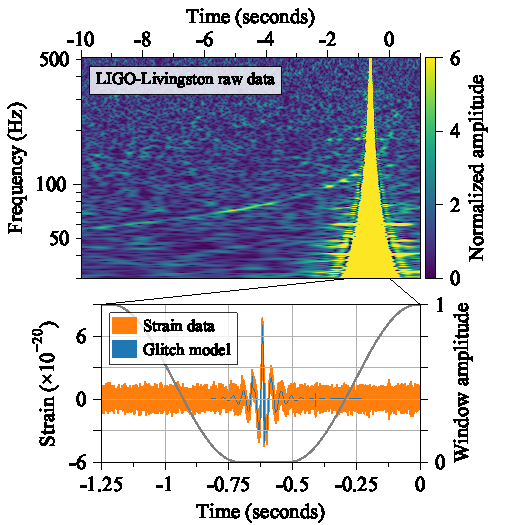
\includegraphics[width=1.0\linewidth]{images/6_earlywarning/gw170817/GW170817_glitch_subtraction.pdf}
    \caption{The Q-scan~\cite{qscan:2004} of the LIGO-Livingston data containing GW170817~\cite{GW170817:2017}, with a very loud wide bandwidth glitch present (top). The glitch was initially subtracted from the data using a windowing function to reduce the amplitude of the data containing the glitch to $0$, this windowing function can be seen as a grey line in the bottom figure. The glitch was also modelled using Bayeswave~\cite{BayesWave:2015} and subtracted from the data to preserve the \gwadj signal power found beneath the glitch, this glitch model (blue line) can be seen overlapping the strain data (orange line) in the bottom figure. This figure has been taken from~\cite{GW170817:2017}.}
    \label{6:fig:gw170817_glitch}
\end{figure}
%
In the fourth observing run we now have well tested and robust search pipelines for \gws and as previously stated, we expect a maximum latency of $20$ seconds post-merger~\cite{PyCBC_Live:2018}, glitches can be auto-gated and BAYESTAR~\cite{BAYESTAR:2016} can produce sky maps in a few seconds.

We can demonstrate the early warning search's efficacy on GW170817. Table~\ref{6:tab:gw170817_early_warning} displays the template bank cutoff frequencies alongside the network SNR of the early warning search searching for GW170817 in the original data and a GW170817-like injection in a representation of the current detector data, also shown is the time pre-merger (warning) at which GW170817 will reach the specified frequency. It can be clearly seen that the SNR of the early warning search hovers around the network SNR threshold of $6$ until the $56$Hz frequency is reach, it is at this point that we can more confidently say that GW170817 would've been seen in early warning, $12$ seconds prior to the merger. The GW170817-like injection into O4 data has very large SNRs in all of the frequencies and we would've observed the $29 \, \text{Hz}$ template with a $67$ second warning.
%
\begin{table}[ht]
    \centering
    \setlength{\tabcolsep}{4pt}
    \rowcolors{4}{white}{lightgray}
    \begin{tabular}{cccc}
        \toprule
        \multicolumn{1}{c}{\textbf{Frequency}} & \multicolumn{2}{c}{\textbf{Network SNR}} & \multicolumn{1}{c}{\textbf{Warning}} \\
        \cmidrule(lr){1-4}
        \textbf{Cutoff [Hz]} & \textbf{Original Data} & \textbf{O4 Injection} & \textbf{Time [s]} \\
        \midrule
        29 & 6.19 & 13.26 & 67 \\
        32 & 5.76 & 18.58 & 52 \\
        38 & 6.11 & 21.96 & 33 \\
        44 & 6.25 & 25.87 & 22 \\
        49 & 6.19 & 24.42 & 17 \\
        56 & 7.04 & 35.24 & 12 \\
        \bottomrule
    \end{tabular}
    \caption{The signal-to-noise ratio values for the \gwadj events with corresponding frequency cutoff found by the PyCBC Live early warning search when searching over the data which contains GW170817~\cite{GW170817:2017} (Original Data) and data which contains a GW170817-like injection into representative data from the fourth observing run (O4 Injection). Also shown is the time before merger in which the event was found (Warning Time).}
    \label{6:tab:gw170817_early_warning}
\end{table}
%
By implementing an early warning search in PyCBC Live we are capable of identifying \gwadj signals before merger. This will aid in localising potentially electromagnetically bright \gwadj signals and inform telescopes of all frequency ranges to capture as much of the electromagnetic counterpart as possible, enabling greater quality multi-messenger astronomy.


\section{\label{6:sec:injection-tests}Testing the early warning search}

To test the capabilities of the early warning search an injection campaign was performed, similar to the injection campaigns performed in the previous chapters~\ref{chapter:4-archenemy} and~\ref{chapter:5-pycbc-live}. The injection set used in this test was custom generated for the early warning search, containing exclusively signals that should be seen by the early warning search.

The intention of this test is to identify any problems with the early warning search as it is current configured. The injections have parameters which should be covered by the template bank but, the full bandwidth SNR of the injection might still be such that it will not be seen by the early warning search.

\subsection{\label{6:sec:injection-set}The distribution of injection parameters}

The injection set contains $32,604$ unique injections placed every ${\sim}100$ seconds, encompassing $3,456,000$ seconds or exactly $40$ days worth of data. The parameters which vary by injection and the ranges in which they vary can be seen in table~\ref{6:tab:ew_inj_params}.
%
\begin{table}[ht]
    \centering
    % \small
    \setlength{\tabcolsep}{4pt}
    \rowcolors{2}{white}{lightgray}
    \begin{tabular}{ccc}
        \toprule
        \multicolumn{3}{c}{\textbf{Variable Parameters}} \\
        \cmidrule(lr){1-3}
        \textbf{Parameter} & \textbf{Value Range} & \textbf{Prior Distribution} \\
        \midrule
        Primary Mass, $m_1$ & $1.0\text{--}3.0$ [$\text{M$_{\odot}$}$] & uniform \\
        Secondary Mass, $m_2$ & $1.0\text{--}3.0$ [$\text{M$_{\odot}$}$] & uniform \\
        Primary Spin z-component, $spin1z$ & $-0.05\text{--}0.05$ & uniform \\
        Secondary Spin z-component, $spin2z$ & $-0.05\text{--}0.05$ & uniform \\
        Distance, $r$ & $10\text{--}1000$ [$\text{Mpc}$] & uniform radius \\
        Phase, $\phi_{c}$ & $0\text{--}2\pi$ & uniform angle \\
        Inclination, $\iota$ & $0\text{--}\pi$ & $\sin$ angle \\
        Polarisation, $\psi$ & $0\text{--}2\pi$ & uniform angle \\
        Right Ascension, $\alpha$ & $0\text{--}2\pi$ & uniform sky \\
        Declination, $\delta$ & $-\frac{\pi}{2}\text{--}\frac{\pi}{2}$ & uniform sky \\
        \bottomrule
        \multicolumn{3}{c}{\textbf{Static Parameters}} \\
        \cmidrule(lr){1-3}
        \textbf{Parameter} & \textbf{Value} & \textbf{} \\
        \midrule
        Waveform Approximant & IMRPhenomXAS~\cite{IMRPhenomXAS:2020} & \\
        Lower Frequency, $f_{lower}$ & 17 [$\text{Hz}$] & \\
        Reference Frequency, $f_{ref}$ & 17 [$\text{Hz}$] & \\
        \bottomrule
    \end{tabular}
    \caption{The parameters used to create the injection set used to test the PyCBC Live early warning search. Variable parameters will be assigned a random value within in the value range distributed across all injections according to the prior distribution. Static parameters are the same for all injections in the injection set. Created using PyCBC~\cite{PyCBC_package:2021}.}
    \label{6:tab:ew_inj_params}
\end{table}
%
These injections are made into simulated coloured noise therefore, no non-Gaussian artefacts exist in the data. The distances generated for each injection are re-scaled after the initial injection set has been created to ensure a uniform SNR distribution of the signals between $12$ and $60$. Therefore the distances might not be exactly uniform in radius and the injection set should be thought to be distributed uniformly in SNR instead.

\subsection{\label{6:sec:results}Results of the early warning injection test}

% TO ADD:
% - Basic stats about results
% - Number of injections
% - Number of candidates found
% - Histogram/Table of candidates per injection
% - SNR distributions for candidates for frequencies
% - 

The parameters of the injection set are chosen such that each injection, if loud enough, can be seen by a template in the early warning search template bank with a minimal match of $0.97$. Each injection can be seen by up to six templates at different frequency cutoffs and with $32,604$ injections in the injection set we could expect a maximum of $195,624$ candidate events in the results. In reality, the lower frequency cutoff templates are likely to not be found for low SNR injections.

We create and run the early warning search on the $40$ days of data containing the injections for both LIGO-Hanford and LIGO-Livingston to find two-detector coincidences. This is consistent with the PyCBC Live early warning search which currently doesn't use Virgo data in the search. The total number of candidates found for all injections is $174,077$, figure~\ref{6:fig:cand_hist} shows a histogram of the number of candidates found per injection.
%
\begin{figure}
    \centering
    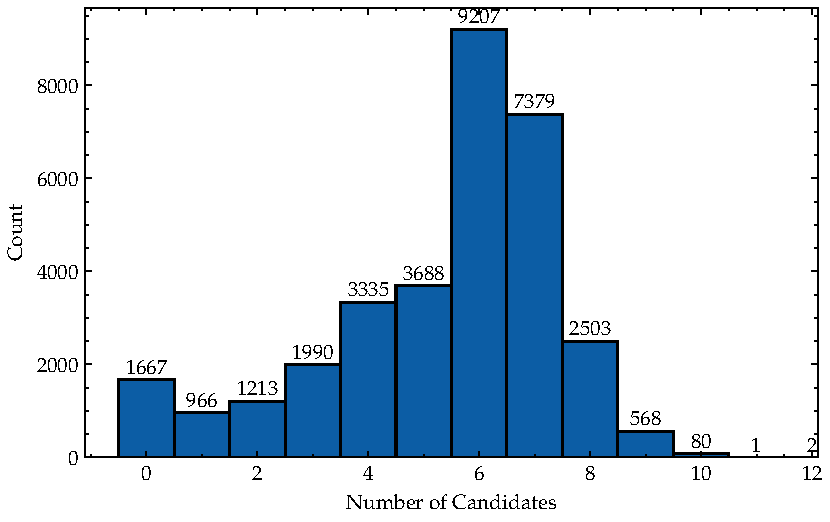
\includegraphics[width=1.0\linewidth]{images/6_earlywarning/results/count_histogram.pdf}
    \caption{A histogram showing the number of injections (Count) found with varying numbers of candidate events (Number of Candidates) by the PyCBC Live early warning search. The exact number of counts is displayed on top of the histogram bars.}
    \label{6:fig:cand_hist}
\end{figure}
%
The histogram shows us a large number of injections which have been found with greater than six candidates, suggesting a problem with the search caused by one or multiple frequency cutoffs being found more than once by the search, the scale of this problem is difficult to see simply from these counts unless the injection is loud enough to be found with all six of the frequencies. Duplicate events for the same frequency cutoff is one of the problems we have identified during this injection study and we will discuss the cause of this problem in the next section, we even have two very rare cases where a duplicate frequency was seen in every single frequency cutoff.

\section{\label{6:sec:identified-problems}False alarms, missed injections and other problems}

Previous injection tests in this thesis were performed to measure sensitivity increases due to significant changes to the \gwadj search pipelines. The injection test performed on the PyCBC Live early warning search was not intended to measure sensitivity increase but to identify problems that might occur with the search that can only be seen by a large number of injections in testing. Performing this injection test will help us identify, investigate and solve problems to the early warning search.

In this section we will identify problems discovered during the injection test. These problems and their impact on the search results will be described and the source of the problem (where identified) will be detailed. Where possible the solution to these problems will also be discussed.

\subsection{\label{6:sec:false-alarms}False-alarm events}

False-alarms are events for which the coincident triggers have originated from non-astrophysical sources to form a candidate found above our statistic threshold. It is easier to identify false-alarm early warning events because those that appear at a lower frequency will not have the corresponding candidates from the next frequencies in the template bank. This is not something the early warning search can take into account in low-latency but it is something that can definitely be used post-detection to confirm the legitimacy of an event.

We can identify false-alarm events in our results by locating candidates which appear with a time of coalescence outside of a short window surrounding any injections times in our injection set.

\subsubsection{\label{6:sec:low-significance-cands}Low significance individual candidates}
%
\begin{figure}
       \centering
    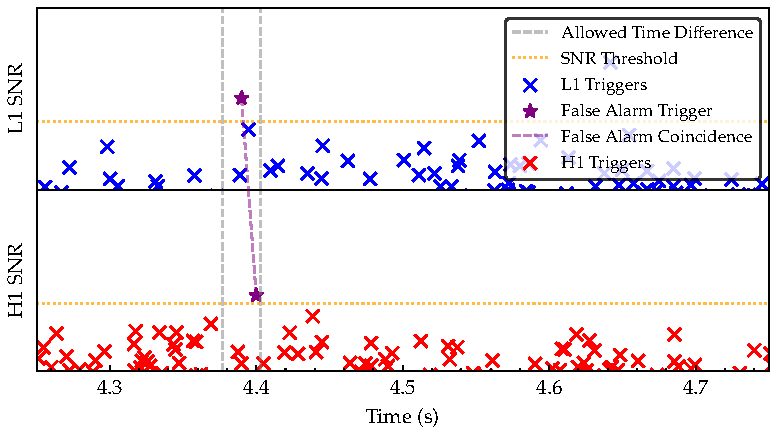
\includegraphics[width=\textwidth]{images/6_earlywarning/identified-problems/low_sig_cands.pdf}
    \caption{An illustration of a coincident candidate being found by the alignment of Gaussian noise triggers in two detectors. The crosses represent the single detector triggers identified by the \gwadj search, triggers found above the SNR threshold can be considered a single detector trigger. Coincident triggers have to lie inside the allowed coincidence window, shows by the grey dashed lines around the L1 trigger.}
    \label{6:fig:low_significance_candidates}
\end{figure}
%
The injection set used in this search was made using a PSD representative of the advanced LIGO noise curve~\cite{aLIGO_design_curve:2018} and therefore is coloured Gaussian noise, not containing any non-Gaussian noise transients. This means that when we identify a false-alarm candidate it has been caused by Gaussian noise triggers aligning in between the two detectors and finding a coincidence, a demonstration of this can be seen in figure~\ref{6:fig:low_significance_candidates}.

The simplest way to identify injections with low significance candidates is to look for injections with single candidates that have frequency cutoffs not equal to the highest cutoff in the template bank ($56 \, \text{Hz}$). In this scenario there are no accompanying higher frequency cutoff candidates and therefore the single event must be due to a random coincidence. Of the ${\sim}32,000$ injections, we observed $99$ with candidates caused purely by the coincidence in Gaussian noise triggers in the two detectors, approximately $0.3\%$ injections.

With more time to dedicate towards investigating the injections found by random noise we could look at the parameters of the candidates and compare them to the injection to see if they match. If they do not, it is likely that the candidate was found due to random noise.

\subsection{\label{6:sec:duplicate-frequency-cands}Finding duplicate frequency cutoff candidates}

% Lay out the problem
%  Injections seen with more than 6 events
%  Injections can only be seen with $6$ max
%  What is happening?
%  Some frequencies are seen twice
%  What?? How can that happen if the search picks the best coincidence in the second that corresponds to the final frequency truncation?

The template bank used by the early warning search is a composite of six template banks. Each template bank contains templates which all end at the same frequency cutoff and is different for each template bank. Therefore, the full template bank contains templates for six different frequency cutoffs.

The time before merger corresponding to each frequency cutoff is then injection specific and you would expect that when the early warning search reaches that time, it would record an event found by a template with the correct frequency cutoff. This then places a maximum number of events found for each injection using the template bank at six events.

We have however, observed injections that have been seen with more than six candidate events. These candidates must have frequency cutoffs equal to one of the six found in our template bank and therefore some frequency cutoffs have been found multiple times for an injection. This should not be possible as the time before merger for the frequency cutoff would correspond to a stride in the early warning search and only the best coincident event can be chosen by the early warning search as a candidate.

\subsubsection{\label{6:sec:cands-across-bounds}Candidates straddling search boundaries}
%  Well, some truncations are close to the boundary
%  Others are across the boundary
%  There is enough lee-way to pick two in two separate seconds
%
\begin{figure}
       \centering
    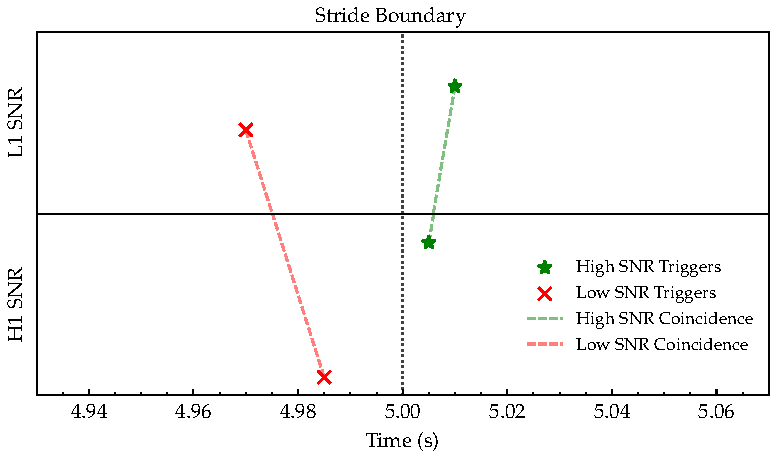
\includegraphics[width=\textwidth]{images/6_earlywarning/identified-problems/cands_across_bounds.pdf}
    \caption{An illustration of two candidate events being found with the same frequency cutoff for a single injection. The red coincidence has lower single detector and coincidence SNR but both are above SNR threshold due to the frequency cutoff template ending very close to the analysis stride boundary, this event is uploaded as a candidate event. The green coincidence is the `proper' coincidence found after the frequency cutoff template has ended and it also uploaded after the first one, leading to two events with the same frequency cutoff being uploaded for one \gwadj signal.}
    \label{6:fig:candidates_across_boundaries}
\end{figure}
%

The early warning search operates on a single second analysis stride, meaning every single second the template bank is matched filtered with the data to discover any \gwadj events. It is possible that the pre-merger time corresponding to a frequency cutoff will lie very near to the boundary between search strides. In this case the search will record an event found in the first stride and will then again record another event in the second stride with the same frequency cutoff.

Figure~\ref{6:fig:candidates_across_boundaries} is a demonstration of this possibility. Either event can have a higher SNR when compared to the other but the two scenarios can be treated differently to prevent some duplicate events being uploaded in the future. If the event found in the first stride has a higher SNR than the second stride we can prevent an upload of the second event (provided the template frequency cutoff is the same)---this is already done by the PyCBC Live Single Detector search~\cite{PyCBC_singles:2022}---but if the event found in the second stride has a higher SNR than the first then we will have to upload two events. We cannot delay uploading the first event.

We found that of the ${\sim}32,000$ injections $13,098$ ($40.17\%$) were affected by this issue, creating at least one extra candidate for a frequency cutoff. This is a massive portion of our injection test and informs us that this is very likely to happen in the future for a real event and therefore, if this does happen it should not be a reason to dismiss a real identification.

% Maybe an example of this happening with a zoom in on the two duplicate frequencies in the track and trigger times, stride boundary time, event time, things like that
% - Example
% - How often it happened
% - Impact

% Total number of injections with duplicate frequencies: 13098
% Fraction of total injections: 40.172984909827015



\subsubsection{\label{6:sec:trigs-across-bounds}Triggers across search boundaries}
%  The search forces a coincidence in the first seocnd and then finds the actual one in the second second
%
\begin{figure}
       \centering
    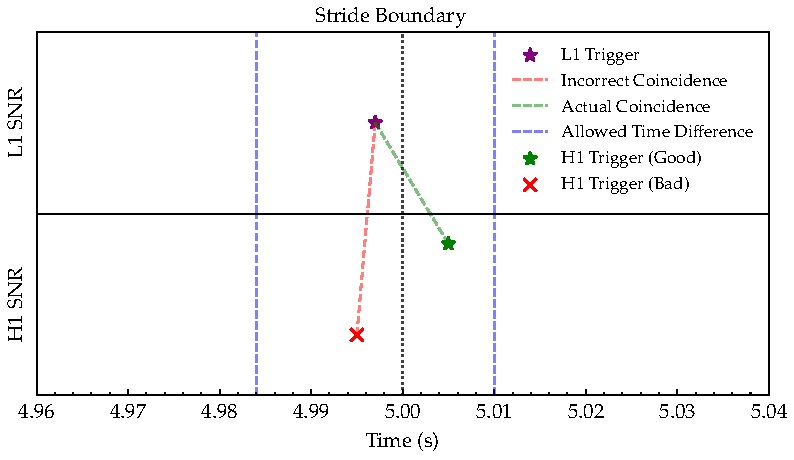
\includegraphics[width=\textwidth]{images/6_earlywarning/identified-problems/trigs_across_bounds.pdf}
    \caption{An illustration of two coincident candidate events being uploaded for the same frequency cutoff. The L1 trigger for the coincidence arrives in the analysis stride and the H1 trigger arrives in the next analysis stride. The early warning search has found a low significance H1 trigger in the first analysis stride and made a low significance coincidence. When the second analysis stride is analysed the correct coincidence will be found and the same L1 trigger is uploaded again with another coincident trigger at the same frequency cutoff.}
    \label{6:fig:triggers_across_boundaries}
\end{figure}
%
The stride boundary can have another effect which causes duplicate frequency events to be uploaded. Coincident triggers between detector 1 and detector 2 have an allowed time difference in each detector to account for the physical light-travel time of the \gw and a smaller amount of computational timing errors. It is possible for the two single detector triggers to appear across a stride boundary.

The trigger will first be seen in detector 1, which will be seen as a highly significant single detector trigger by the early warning search, where it will attempt to match with a coincident trigger in the other detector. As previously mentioned, this could be Gaussian noise which happens to match well enough for a low-significance coincidence to be made. When detector 2 records the trigger in the next stride the early warning search will create the actual significant coincident event using the same detector 1 trigger twice. Therefore, we will get two candidate events at the same final frequency cutoff with one being less significant than the other. A demonstration of this case is seen in figure~\ref{6:fig:triggers_across_boundaries}. This is unavoidable, we need the light travel time in the ranking statistic and this can straddle two strides.

% Example once again of the same trigger being used for both events? H1 SNR the same, L1 snr different (much lower and much higher)
% - Example
% - How often it happened
% - Impact




\subsection{\label{6:sec:outside-coinc-window}Coincident triggers outside the light-travel time}
%
\begin{figure}
    \centering
    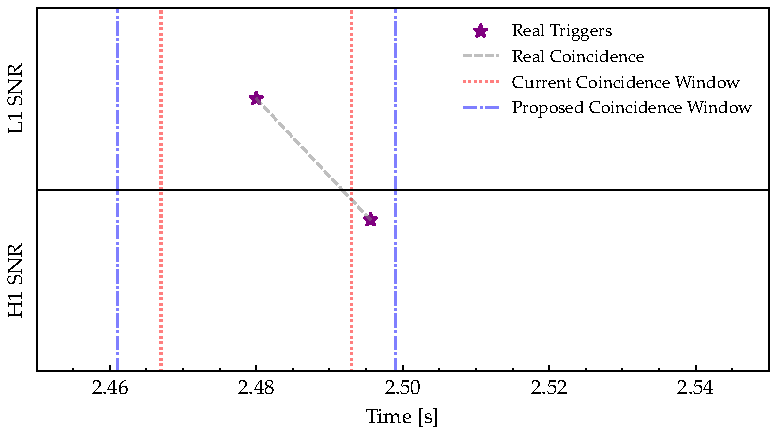
\includegraphics[width=\textwidth]{images/6_earlywarning/identified-problems/outside_coinc_window.pdf}
    \caption{An illustration of two single detector triggers being found outside the allowed coincidence time difference window. The current coincidence window shows the triggers falling outside the window and therefore the search does not form a coincidence. With the new proposed coincidence time window the coincidence would be found.}
    \label{6:fig:outside_coinc_window}
\end{figure}
%
% What is the broad problem?    
% What are some ways it manifests
% How can we solve this problem
%  Coinc Window - Fairhurst
%  PhaseTD tuning for statistic
%  Sample rate issue

A problem that we have identified in the analysis of the results is valid candidates events being missed due to the coincident triggers falling outside of the allowed coincidence time window. The coincidence time window is a sum of the light-travel time and a computational timing error allowance. The two LIGO detectors are separated by a straight line through the Earth $3002$ kilometers long. Given the speed of light, c $= 300,000$ km/s, there is a $0.01$ window and the current addition for errors is $0.003$ seconds, giving a total allowed coincidence timing window of $0.013$ seconds. How then, is it possible for our completely valid coincident triggers to lie outside of this window?

\subsubsection{\label{6:sec:timing_error}Timing accuracy error}

Firstly, as described in~\cite{Fairhurst:2010}, the accuracy of the candidate time in a detector can be determine by,
%
\begin{equation}
    \sigma_{t} = \frac{1}{2\pi\rho\sigma_{f}}
    \label{6:eqn:timing_acurracy}
\end{equation}
%
where the timing accuracy, $\sigma_{t}$, is inversely proportional to the SNR, $\rho$, and the effective bandwidth of the source, $\sigma_{f}$ which is defined as
%
\begin{equation}
    \sigma_{f}^2 = \left(\int^{\infty}_{0} df \frac{f^{2}|\hat{h}(f)|^{2}}{S(f)}\right) - \left( \int^{\infty}_{0} df \frac{f|\hat{h}(f)|^{2}}{S(f)}\right)^{2} .
    \label{6:eqn:eff_bandiwdth}
\end{equation}
%
where the waveform $\hat{h}$ is normalised such that $\int \frac{|\hat{h}(f)|^{2}}{S(f)}df = 1$; we use the same PSD to normalise that has been used throughout the injection study. As shown in Table 1. of~\cite{Fairhurst:2010}, the timing error for a binary neutron star system in an advanced LIGO configuration with a BNS range of $160$ Mpc is $0.46$ms. Negligible when compared to our light-travel time of $10$ms. We can approximately calculate the timing accuracy of the early warning templates using equations~\ref{6:eqn:timing_acurracy}\&~\ref{6:eqn:eff_bandiwdth}, where the \gwadj strain term, $|h(f)|$, is assumed to be equal to the inspiral frequency evolution of a binary neutron star signal, $f^{-\frac{7}{6}}$. The estimated effective bandwidths and timing accuracy errors can be seen in table~\ref{6:tab:timing_errors}.
%
\begin{table}[ht]
    \centering
    \setlength{\tabcolsep}{4pt}
    \rowcolors{3}{white}{lightgray}
    \begin{tabular}{ccc}
        \toprule
        \textbf{Frequency [Hz]} & $\sigma_{f}$ [Hz] & $\sigma_{t}$ [ms] \\
        \midrule
        29 & 3.38 & 5.89 \\
        32 & 4.19 & 4.75 \\
        38 & 5.79 & 3.44 \\
        44 & 7.37 & 2.70 \\
        49 & 8.68 & 2.29 \\
        56 & 10.51 & 1.89 \\
        1024 & 90.05 & 0.22 \\
        \bottomrule
    \end{tabular}
    \caption{The effective bandwidth, $\sigma_{f}$, and timing accuracy error, $\sigma_{t}$, for the frequency cutoffs (Frequency) found in the early warning template bank as well as the full bandwidth frequency ($1024 \, \text{Hz}$).}
    \label{6:tab:timing_errors}
\end{table}
%
Using an SNR of $8$ (and a lower frequency of $17$ Hz) yields timing errors from $5.89$ to $1.89$ milliseconds for the early warning frequency cutoffs, where higher frequencies have smaller timing errors. The current allowed error is $3$ milliseconds therefore we do not expect to miss candidates from the $44$, $48$ and $56 \, \text{Hz}$ templates. The window does need to be widened to ensure we aren't missing $29$, $32$ and, $38 \, \text{Hz}$ frequency cutoff templates. This could be done on a template dependent basis, with a timing accuracy error dependent on the frequency cutoff. When we investigate the injections which have missing frequencies we get the following counts per frequency cutoff: $29 \, \text{Hz} = 0$ (We do not distinguished between missed and not found for the first frequency cutoff), $32 \, \text{Hz} = 288$, $38 \, \text{Hz} = 162$, $44 \, \text{Hz} = 132$, $49 \, \text{Hz} = 168$, $56 \, \text{Hz} = 140$, therefore the timing window needs to be widened for all frequency cutoffs.

\subsubsection{\label{6:sec:sample_accuracy}Sampling accuracy}
% PyCBC Live Full Bandwidth Sample Rate
%  Why does it need a high sample rate
% PyCBC Live Early Warning Sample Rate
%  Why is it lower
%   To capture the f_final in the nyquist
%  Why isn't it even lower?
%   You lose out on time and phase resolution
%  How is this affecting our search
%   Triggers in between two samples can be found outside the coincident time window

The PyCBC Live Full Bandwidth search uses a sample rate of $2048$Hz to capture binary neutron star signals which can merge even above the $1024$Hz Nyquist frequency with the greatest accumulated SNR. The PyCBC Live Early Warning search uses a sample rate of $256$Hz, giving a Nyquist frequency of $128$Hz. The highest frequency cutoff templates are at $56$Hz so these can all be fully captured with a sample rate of $128$Hz. The sample rate is increased to $256$Hz to ensure we have a greater time resolution and phase accuracy, a sample rate of $128$Hz has a time between samples of $7.8$ms which is close to our allowed light-travel time.

We have seen that the $256$Hz sample rate might still provide an issue with timing accuracy and the current allowed coincidence time window. With a time between samples of $3.9$ms a trigger in another detector $3$ samples later will be within the allowed window of $13$ms but being $4$ samples later equals a time difference of $15.6$ms; falling outside the window. We have seen cases whereby increasing the sample rate of the early warning search will locate a coincidence within the time window where previously it was seen outside. Increasing the sample rate however, does increase the computational cost of the search with no increase in event SNR or new events provided.

\subsubsection{\label{6:sec:ew_phasetd}Early warning tuned PhaseTD histogram}
% Great, we've made the window bigger
% What? It still won't work? Why not?
% PhaseTD File
%  What is it?
%  How is it made?
%  How is it tuned?
%  Does it take into account time windows outside the 13ms? (no)

By increasing the allowed coincidence time window we will allow the early warning search to make those initial coincident triggers which share the same template parameters and are physically possible (when accounting for timing accuracy error). However, we will face another problem where the coincident ranking statistic used by the early warning search will consider these events to have a very low signal rate. The coincident ranking statistic used by the early warning search is \verb|phasetd| (phase-time delay) and is used to assess the coincidence likelihood between two triggers from different detectors.

For a two detector coincidence the likelihood value is found by sampling from a pre-created \verb|phasetd| 3-dimensional histogram in amplitude, time and phase space. This file is created using by simulating \gwadj signals from an isotropic distribution of sources. Each signal is assigned a random sky location (right ascension, declination and inclination) and polarisation, then the response in each detector is calculated to determine the sensitivity to the signal in both detectors. From this response we can get the signal amplitudes, time delays and phases shifts for each detector. For the pair of detectors the time delay, phase differences and relative signal amplitudes are then binned into discrete bins which represent different combinations of amplitude, time and phase difference.

The size of the bins is determined by the allowed uncertainties in timing, phase and SNR. Additionally there is a restriction in the allowed range of SNR ratios to avoid storing bins for extreme values. After this, smoothing is performed between nearby bins and the final histogram is produced. Within the search, time difference, phase difference and amplitude ratios are then used to sample from this histogram to calculate the likelihood of the three parameter combination.

Currently the allowed time window uncertainty is $1$ms which determines the bin size and while a large time difference between two triggers is allowed, 


The allowed time window used when creating the histogram is currently $1$ms, this determines the bin size so with a large number of bins we can sample from the histogram with a large time difference value. However, the monte carlo simulation to create the histogram will not place any simulated injections in these bins due to not accounting for a large enough timing error. Therefore, when we sample from the histogram with large time difference we will receive very low value of the signal rate. The timing accuracy error will need to be taken account explicitly in the time difference on both trigger times.

Another improvement that can be made in the generation of the \verb|phasetd| statistic files is including the sample rate of the search as a parameter. For a monte carlo simulation the trigger time differences are as accurate as a \verb|float64| parameter can be. Whereas the timing difference between triggers in the PyCBC Live search will only take discrete values of the time difference dependent on the sample rate, for example, the early warning search has a sample rate of $256$Hz and therefore the time difference between samples is $0.00390625$ seconds or approximately $3.9$ milliseconds. Therefore our \verb|phasetd| file will only ever been sampled from using time difference that are n-multiples of this time between samples. We can create \verb|phasetd| files with bins in the time difference parameter space which represent the sample rate of the search and therefore can be sampled more accurately.

\subsubsection{\label{6:sec:missing-cands}Missing candidates}
%
\begin{figure}
       \centering
    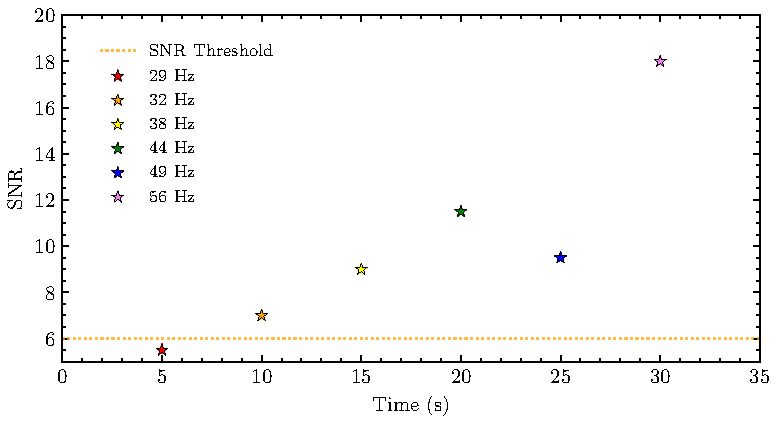
\includegraphics[width=\textwidth]{images/6_earlywarning/identified-problems/non_mono_snr.pdf}
    \caption{An illustration of the expected and SNRs for the case where one of the event's coincident triggers have fallen outside of the coincident timing window. In the first case we see a missing frequency in the SNR evolution (indicated by the red cross), in the second case we see a non-monotonic increase in SNR where the search has found a low significance event to `fill' the gap (shown by the orange star).}
    \label{6:fig:non-monotonic-snr}
\end{figure}
%
% - Example
% - How often it happened
% - Impact

The most obvious indicator that the search has failed to find a coincidence due to the coincident trigger time difference falling outside the coincidence allowed timing window is that injections have `missing' events in the frequency evolution. We would expect to see a sequence of events for each injection when the starting frequency is not the greatest frequency cutoff in the bank. For example, if we saw a real \gwadj signal whose initial event has a frequency cutoff of $29$Hz then we would expect to find the $32$, $38$, $44$, $49$ and $56$Hz candidate events shortly following. If we fail to see the $32$Hz event but we still see the following events then we know that something has broken in the early warning search.

We know that the $32$Hz triggers exist but they fall outside the allowed coincidence timing window and therefore a coincident event was never formed. The early warning search will output files containing all the single detector triggers found which we can use to identify the missing coincidence. Figure~\ref{6:fig:missing-freq-eg} shows an example of an injection which has been found with all but $1$ final frequency cutoff template. 
%
\begin{figure}
    \centering
    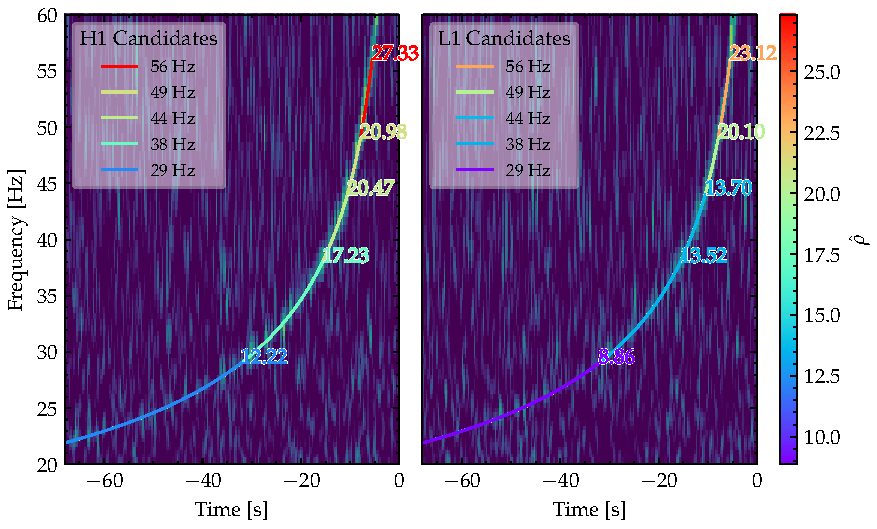
\includegraphics[width=1.0\linewidth]{images/6_earlywarning/stories/missing_freqs_example.pdf}
    \caption{An example of a \gwadj injection seen by the PyCBC Live early warning search with a missing template with frequency cutoff $32 \, \text{Hz}$.}
    \label{6:fig:missing-freq-eg}
\end{figure}
%
To verify the time difference problem we investigated the expected network SNRs for this injection at each final frequency cutoff in both a noiseless and expected noise regime (not performed using the PyCBC Live search). The values for these can be seen in table~\ref{6:tab:noise_snrs}.
%
\begin{table}[ht]
    \centering
    \setlength{\tabcolsep}{4pt}
    \rowcolors{2}{white}{lightgray}
    \begin{tabular}{ccc}
        \toprule
        \textbf{Frequency Cutoff [Hz]} & \textbf{Noiseless SNR} & \textbf{Noisy SNR} \\
        \midrule
        29 & 16.43 & 15.38 \\
        32 & 19.16 & 17.95 \\
        38 & 24.00 & 21.50 \\
        44 & 28.11 & 25.26 \\
        49 & 31.04 & 27.94 \\
        56 & 34.48 & 29.02 \\
        \bottomrule
    \end{tabular}
    \caption{The expected signal-to-noise ratios in both noiseless and noisy data for the \gwadj injection shown in figure~\ref{6:fig:missing-freq-eg}. The noiseless SNR has been calculated by taking the un-normalised matched-filter of the template with itself~\cite{Brown_Thesis:2004}. The noisy SNR has been calculated by matched-filtering the template with the injection that has been injected into simulated \gwadj data.}
    \label{6:tab:noise_snrs}
\end{table}
%
We can clearly see that we are expecting to see a large network SNR for the $32$Hz case which isn't recovered by the search. Next we are able to re-run the early warning search using a template which perfectly describes the injection parameters and in this case we still fail to recover the candidate event but, we can look into the trigger files to identify the single trigger found by both searches with the same template above the SNR threshold. We find a H1 trigger with SNR $14.55$ and an L1 trigger with SNR $12.38$ (giving a network SNR of $19.11$) and when the time difference between triggers is calculated we get $0.015625$ seconds, greater than the currently allowed $0.013$ seconds. 

We can then perform another search with a sample rate of $2048$Hz, which doesn't find a coincidence but has a smaller time difference of $0.0146$ seconds (still outside the window) proving that the time accuracy error is playing a part and it isn't simply a sampling inaccuracy. When performing a final search in which we expand the allowed coincidence timing window by $10$ms (this can be tuned in the future) we successfully recover all $6$ events for this injection.

However, we still need to investigate how the \verb|phasetd| ranking statistic has responded to the highly unlikely time difference. We calculate the signal rate using
%
\begin{equation}
    \log(r_s) = \frac{R - \hat{\rho}_{H}^{2} + \hat{\rho}_{L}^2}{2}
\end{equation}
%
where R is the event's ranking statistic value and $\hat{\rho}_{H}$ and $\hat{\rho}_{L}$ are the single detector new SNRs. We recover a signal rate using the same \verb|phasetd| histogram being used by the PyCBC Live search of $-24.70$. This is extremely low and therefore the signal is being considered as extremely unlikely but, the SNRs of the signal are so high such that this is compensated for and the ranking statistic value found by the search overall is around $17.77$, quite significant. This points to issues surrounding the \verb|phasetd| histogram file that still needs to be fixed.

We find that $873$ injections are missing at least one candidate in the frequency evolution, this represents $2.68\%$ of all injections in our injection set. We note that we will only be counting injections which see more than one candidate event and where the candidate missing frequency isn't the lowest frequency in the evolution. If the missed frequency was the $56 \, \text{Hz}$ frequency but this was the only frequency cutoff seen for that injection then we would not count it as a missed frequency. If the missed frequency is the lowest frequency in the evolution, for example $29 \, \text{Hz}$, then we are just assuming that the $29 \, \text{Hz}$ did not have enough SNR to be seen and wasn't `missed' in this context. A more detailed analysis is possible using the expected SNRs of the frequency cutoffs.

\subsubsection{\label{6:sec:non-mono-snr}Non-monotonic SNR evolution}
% - Example
% - How often it happened
% - Impact

Another manifestation of the timing accuracy error is the possibility for the missing frequency to be found but with a SNR not following a monotonic SNR increase across the entire injection event timeline. A demonstration of this can be seen in figure~\ref{6:fig:non-monotonic-snr} and an example of this happening for an injection in our early warning search can be seen in figure~\ref{6:fig:non_mono_eg}.
%
\begin{figure}
    \centering
    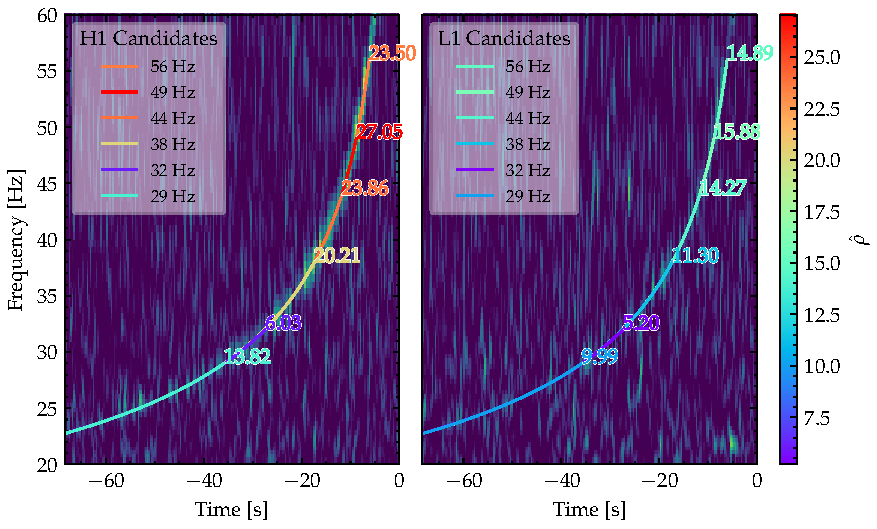
\includegraphics[width=1.0\linewidth]{images/6_earlywarning/stories/non_mono_example.pdf}
    \caption{An example of a \gwadj injection that has been found with a non-monotonically increasing signal-to-noise ratio between successive frequency cutoffs. The $32 \, \text{Hz}$ frequency cutoff \gwadj template has been seen with a lower SNR in the H1 and L1 single detector searches than the $29 \, \text{Hz}$ frequency cutoff template. This is caused by the actual $32 \, \text{Hz}$ template coincident triggers being found outside the allowed coincidence timing window.}
    \label{6:fig:non_mono_eg}
\end{figure}

It can be seen that the $32$Hz has been found by the search for this injection but with a much lower SNR than expected and not following the monotonic SNR increase that we would expect. When investigating the triggers found we can see that the search has managed to find a low-significance trigger within the coincidence time window and has managed to form a coincidence with low SNR, similar to the low significance candidates described in section~\ref{6:sec:low-significance-cands} but where one trigger is actually real. Looking into the single detector trigger files we can once again find the coincident trigger pair that should've been made if the coincidence timing window was larger and when running the search over this injection with the larger coincidence time window we find all $6$ events for this injection with the expected SNR.

We find that $997$ injections had non-monotonically increasing SNR between all successive frequency cutoffs. However, we expect a number of injections to have non-monotonically increasing SNRs due to Gaussian noise in the detector influencing the SNR values recovered for some templates. Therefore, we only count injections in which the drop between successive SNRs is greater than $5\%$ of the previous frequency cutoff template's SNR. When applying this limit we obtain only $120$ injections with non-monotonically increasing SNR ($0.37\%$).

% Total number of injections with non-monotonic SNRs: 997
% Fraction of total injections: 3.0579070052754265
% Total number of injections with non-monotonic SNRs above threshold: 120
% Fraction of total injections: 0.368052999631947



\section{\label{6:sec:conclusion}Conclusion}

We have described the PyCBC Live early warning search and how it is used to enhance multi-messenger astronomy by providing early warning of \gwadj signal mergers to allow electromagnetic telescopes the ability to prepare for incoming counterparts to \gwadj signals in the electromagnetic observation regime.

We have performed a injection study using the early warning search to identify any potential problems with the search that might negatively affect any results from real events in the future. From this study we have identified three main categories of problem, relating to low significance Gaussian noise events, analysis stride boundaries interrupting analysis and producing duplicate events and, timing accuracy errors preventing the coincidence of two real single detector triggers being formed. We have provide the cause of these problems alongside illustrations and examples of cases in which they have occurred during our test. Further information has been provided for the timing accuracy error problem on solutions as well as further consideration (phase-time delay ranking statistic) for problems that need to be fixed in the future to ensure correct operation of the early warning search.

In conclusion, the early warning search is more than capable of observing \gwadj signals tens of seconds prior to the merger of the \gwadj event. We are able to disseminate information about this event to the international science community however, there are problems with the search that have the potential to negatively affect the results of real events found in the future.















% \section{\label{6:sec:potential-improvements}Potential Improvements}

% While I am not including the improvements that are suggested here into the early warning search, due to time constraints, I will delve into some of the improvements that can be made and the positives and negatives of their effect upon the search.

% \subsection{\label{6:subsec:ranking-statistic}Additions to the Ranking Statistic}

% The ranking statistic, as mentioned in previous chapters, is the way in which we can evaluate the likelihood of a particular candidate being 'real'. Therefore, if we include more and more components into the ranking statistic, we can build up a more confident picture of what determines the realness of a candidate and whether we should share this candidate with the wider research community.

% The current ranking statistic used by the early warning search is very very simple, in the single detector triggers it is a simple ranking of `newsnr' where the chi squared tests are used to determine if the correct amount of power is located in each bin of the template. For the coincident ranking statistic we used `phasetd' which is another simple check of phase and amplitude consistency between detectors in the time domain.

% We have two careful consideration with regards to the ranking statistic. Number 1, computation time and avoiding introducing any lag into the early warning search. The early warning search has a stride length of one second, if any complicate computational steps are added to the ranking statistic we might risk delaying any detected early warning candidates and defeating the purpose of the search. Number 2, eliminating potential candidates before we send them out. No ranking statistic is perfect and the resulting quantitative analysis from the ranking statistic, the false alarm rate, is cut off at a human chosen number (typically one or two per year). Therefore, if we introduce more and more complicated components to the ranking statistic we might risk eliminating early warning candidates which don't meet the PyCBC threshold of a confident event but, other non-IGWN people might take that risk and perform their observations or analyses using our non-confident predictions. Therefore we might actually want to either keep our ranking statistic fairly simple, to not lose these rare events, or lower our threshold when using a complicated ranking statistic so that we still disperse these events but with a big asterisk that we do not think they're real and might fall below someone's threshold.

% If we wanted to make some improvements to the ranking statistic we can consider including some early warning specific information which we would know at the time of the search. This is either historical information based on the previous results produced by the early warning search, something similar to the template fits used in offline and the full bandwidth live search, or maybe even an astrophysical analysis of what we expect to see based on a population model, something like the KDE statistic (I think??).

% Real time information that could be used in the search pertains to the state of the detector at that very time, inclusion of iDQ and DQ, it could also include the detected candidates that have already been found and are being kept in a rolling buffer. We do expect that for a real \gwadj signal that can be found in early warning, to see a cascade of events uploaded with subsequent frequencies getting higher and higher. We could check if any previous frequencies were uploaded, or in posterity whether any further frequencies were uploaded. If a candidate has been found first at 38Hz, does this mean we missed a 29Hz and a 32Hz signal or were these too quiet? Can we spin up a small job to do a deep dive on whether these lower frequencies are in-fact there? There are many small changes that can be made to the early warning search to iteratively improve upon it and make it more robust and confident in detecting these rare events.

% \subsection{More Frequency Truncations per Template}
% We currently have five frequency truncations per template in our bank. This is to prevent a massive amount of templates in the bank and is a good balance for shorter templates which might transition between frequency truncations faster than the search stride time when reaching higher frequencies.

% We could produce a template bank with a number of different configurations and requirements:
% - Greater number of frequency truncations for all templates
% - Template dependent frequency truncations, longer duration templates will have more frequency truncations
% - Equal truncations per template but sigma dependent spacing
% - Time before merger spacing of templates, 1 template every 3/4/5 seconds or something. Or 8 templates per duration

% \subsection{Great parameter distribution in template bank}
% The distribution of template parameters is conservative in the early warning search. We only want to find and report on signals that have a potential electromagnetic counterpart however our template bank could be too conservative and by allowing a greater parameter distributions of templates we could discover some templates on the edge of the bank with a greater SNR or templates that previously we wouldn't have seen.

% To test a larger template bank we would need to produce an injection set containing a larger number of signals that we might consider EM bright, recent literature has highlighted previously unknown signals that could have EM counterparts~SOURCE SOURCE SOURCE.

% \subsection{Adding Spins to the Template Bank}
% Currently the template bank is limited to aligned 0 spin templates. We tested the search with an injection set of slightly spinning templates and this spin will not be seen by the early warning search. It is known that neutron stars have theoretical spins up to +-0.4 so there is a potential for us to be missing spinning neutron star signals and therefore precessing signals in our search. While precessing signals are more difficult to see due to difficulties in including the many more parameters requires this search is very light weight currently and more computing power could be added to balance out the lag increase from introducing more complicated template banks to the search.

% \subsection{Approximants with greater physics}
% Due to the small number of templates and them being only generated once for the live search we might be able to use a more expensive template model which includes physics which can capture some unique properties of low mass signals like tidal deformation or orbital eccentricity, using a better equation of state, higher order modes or high order PN terms.






%%%%%%%%%%%%%%%%%%%%%%%%%%%%%%%%%%%%%%%%%%%%%%%%%%%%%%
\section*{Appendix}
\section{Problems Faced when producing Injection Data}

One of the problems experienced while doing the data analysis of this project is an issue caused by the method of creating the data initially. The PyCBC function used was \verb|pycbc_condition_strain| which takes an input for the power spectrum density of the noise you with to simulate. We used an analytical PSD (NAME, REF, CITE) which produced discontinuities at the boundaries between our data segments and therefore negative effects on the matched filtering being performed by the live search. An example of one of these discontinuities and an injection missing some candidates can be seen in figure~REMOVED.
% %
% \begin{figure}
%        \centering
%     \includegraphics[width=\textwidth]{}
%     \caption{}
%     \label{fig:ew_boundary_problem}
% \end{figure}
% %
The bug can be explained by the analytical PSD not cutting off naturally when tending towards 0Hz and instead takes on values incompatible with a real PSD. This 'bug' has since been reported and a user-based solution has been found, to include a new argument to condition strain to perform a highpass on all frequencies below 10Hz. Unfortunately we did include a highpass argument on the data originall when creating the data but it was the wrong one!

Since discovering this boundary issue the same data has been re-created with the same PSD but the correct highpass argument has been given and therefore the boundary issue has been resolved and we have re-performed the initial data analysis with the new data.


\section{Existing Limitations}

\subsection{Computational Limitations}

The early warning search is heavily optimised to the point it runs on a single dedicated machine with $10$ processes and $2$ threads per process. Just as the with full bandwidth search, the template bank is parallelised over these processes using MPI so each process will be performing the matched filter for only a few hundred templates before the message passing interface receives all the results and the coicidences are found by the rank 0 process. The search can be badly affected by other processes running on the same machines so this machine is exclusively used by the PyCBC Live early warning search.

The search can suffer heavily from other non-PyCBC processes such as file storage, data frame delivery or GraceDB uploads. These can be mitigated slightly with reserved local storage on the dedicated machine or subprocess multiprocessing for the GraceDB uploads so the search isn't waiting on GraceDB to continue processing, especially at times where multiple events are being uploaded for a single signal and across multiple searches from other pipelines.

Another consideration and computational limitation is the limit in introducing new computationally complex processes to the search that might introduce lag to individual processes. Potential changes to the ranking statistic could be challenging to implement without slowing down individual processes or the coincidence rank 0 process. With a data stride of one second we need to be sure that the data processing for the current second is completed before the next second of data arrives or we will slowly build up a debt of data which the search can never get on top of.

